\clearpage
\setcounter{page}{1}
\maketitlesupplementary

\renewcommand{\thesection}{S\arabic{section}}
\renewcommand{\thesubsection}{S\arabic{section}.\arabic{subsection}}
\setcounter{section}{0}



\section{Detailed Preliminaries}
\label{supp:pref_optim}

Building upon the probabilistic formulation introduced above, preference optimization aims to align the conditional policy $\pi_{\theta}(y|x)$ with desired responses based on pairwise preference supervision. 
This paradigm originates from reinforcement learning from human feedback (RLHF) \cite{Christiano2017RLHF}, 
where a reward model $r(x,y)$ is learned to reflect human preference and the policy is optimized with reinforcement learning algorithms such as PPO \cite{Schulman2017PPO}. 
Following the Bradley--Terry model \cite{Bradley1952BT}, the probability of preferring one response $y$ over another $y'$ given the same input $x$ is modeled as
$
P(y \succ y'|x) = \sigma(r(x,y) - r(x,y')) ,
$
where $\sigma(\cdot)$ denotes the sigmoid function. 
Given the true reward model $r(x,y)$, RLHF seeks to maximize the expected reward while constraining deviation from a reference policy $\pi_{\text{ref}}$, formulated as $
\max_{\theta} \; \mathbb{E}_{x,y\sim\pi_\theta} [r(x,y)] - \eta^{-1} \, \mathbb{E}_{x} [\mathrm{KL}(\pi_\theta(\cdot|x) \| \pi_{\text{ref}}(\cdot|x))],
$
where $\eta$ controls the trade-off between reward maximization and policy regularization. 


Rafailov \textit{et al.} \cite{rafailov2023direct} showed that this optimization admits a closed-form solution $
\pi^{*}(y|x) \propto \pi_{\text{ref}}(y|x)\exp(\eta\, r(x,y))$,
which directly connects policy improvement with the reward difference between preferred and dispreferred responses. To remove the explicit reward model, DPO reformulates this closed-form expression as a supervised learning objective. 
Given a preference dataset $\mathcal{D}=\{(x^{(i)},y_w^{(i)},y_l^{(i)})\}_{i=1}^{N}$, where $y_w$ and $y_l$ denote the preferred and dispreferred responses for input $x$, the DPO loss is
\begin{equation}
\small
\begin{aligned}
&\mathcal{L}_{\text{DPO}}(\pi_\theta; \pi_{\text{ref}}) 
= -\mathbb{E}_{(x,y_w,y_l)\sim\mathcal{D}} \\&\Bigg[
\log \sigma \Big(
\eta^{-1} \log \frac{\pi_\theta(y_w|x)}{\pi_{\text{ref}}(y_w|x)}
- \eta^{-1} \log \frac{\pi_\theta(y_l|x)}{\pi_{\text{ref}}(y_l|x)}
\Big) \Bigg].
\end{aligned}
\label{eq:dpo_loss}
\end{equation}
This formulation directly calibrates the relative log-likelihood between preferred and dispreferred responses, providing a stable and reward-free approach for preference-based alignment of large multimodal models.

% From main paper^
% ---------------

% \subsection{Causal Counterfactual Learning}
% \label{supp:pref_optim}




%\section{Preliminary of Causal Counterfactual Learning}
%\label{supp:causal}

\iffalse
\begin{definition}[Causal reward]
    Given background $B{=}b$ and the ensemble mediator $E$, let $e$ denote the factual embedding and $e^\star$ the counterfactual embedding that would have been obtained under the counterfactual background. 
The total indirect effect on reward is defined as
\begin{equation}
\label{eq:tie-reward-def}
r_{c}(x,y)
\;:=\; R_{b,e}(x,y)\;-\;R_{b,e^\star}(x,y).
%\footnote{We use $x$ to represent input image $I$ to keep the same form as the standard DPO, where clinical query is omitted for simplicity.}.
\end{equation}
\end{definition}
\fi

\section{Proof of Theorem \ref{thm:tie_convergence}}
\label{supp:theory}

\noindent
We provide theoretical analysis showing that, even when the reference policy $\pi_{\text{ref}}$
is biased by observational shortcuts, causal preference optimization provably converges closer to the causal-optimal policy and achieves vanishing causal preference regret.


\begin{assumption}[Boundedness and realizability]
\label{ass:bounded}
The reward functions are bounded by $R_{\max}$,
the bias magnitude satisfies $\|\delta\|_\infty \le \varepsilon$,
and the learning rate $\eta$ is sufficiently small
so that multiplicative-weight updates remain stable.
\end{assumption}

%---------------------------------------------
% Lemmas
%---------------------------------------------
\begin{lemma}[Bias propagation under exponential tilting]
\label{lem:bias}
For a fixed $(x)$, let
$q_c(y)\propto \pi_{\mathrm{ref}}(y\mid x)\,e^{\eta r_c(x,y)}$
and
$q_o(y)\propto \pi_{\mathrm{ref}}(y\mid x)\,e^{\eta(r_c(x,y)+\delta(x,y))}$.
If $\|\delta\|_\infty\le \varepsilon$, then
\[
\mathrm{KL}(q_o\|q_c) \le 2\eta\,\varepsilon,
\qquad
\|q_o-q_c\|_{\mathrm{TV}} \le \sqrt{\eta\,\varepsilon}.
\]
\end{lemma}

\begin{proof}
Let $Z_c=\sum_y \pi_{\mathrm{ref}}(y\mid x,e)e^{\eta r_c(x,y)}$ and 
$Z_o=\sum_y \pi_{\mathrm{ref}}(y\mid x)e^{\eta(r_c(x,y)+\delta(x,y))}$ 
be the normalizing constants for $q_c$ and $q_o$, respectively.  
By definition of the log-density ratio,
\[
\log\frac{q_o(y)}{q_c(y)}
= \eta\,\delta(x,y) + \log\frac{Z_c}{Z_o}.
\]
Since $\delta$ is bounded by $\varepsilon$, we have
$|\eta\,\delta(x,y)|\le \eta\varepsilon$.  
To bound the partition term, note that
\[
e^{-\eta\varepsilon} \le \frac{Z_c}{Z_o} \le e^{\eta\varepsilon}
\quad \Rightarrow \quad
\big|\log\frac{Z_c}{Z_o}\big| \le \eta\varepsilon.
\]
Therefore, the log-density ratio satisfies
$|\log(q_o/q_c)| \le 2\eta\varepsilon$.
Integrating over $q_o$ gives
$\mathrm{KL}(q_o\|q_c)\le 2\eta\varepsilon$.
Applying Pinsker’s inequality,
$\|q_o-q_c\|_{\mathrm{TV}}\le \sqrt{\tfrac{1}{2}\mathrm{KL}(q_o\|q_c)} \le \sqrt{\eta\varepsilon}$.
\end{proof}


\begin{lemma}[Expected one-step improvement]
\label{lem:onestep}
Under Assumption~\ref{ass:bounded},
the causal preference optimization updates
\[
\pi_{t+1}(y\mid x)
\propto
\pi_t(y\mid x)
\exp\!\big(\eta\,\widehat r_c^{(t)}(x,y)\big)
\]
satisfies
\[
\small
\begin{aligned}
\mathbb{E}\!\left[\mathrm{KL}\big(\pi_{t+1}\|\pi_c^\star\big)\mid\pi_t\right]
&\le
\mathrm{KL}\big(\pi_t\|\pi_c^\star\big)
-
\eta\,\mathbb{E}_{x,e}\!\big[\mathrm{Var}_{\pi_t}(r_c(x,\cdot))\big]\\
&\quad
+ O(\eta^2R_{\max}^2).
\end{aligned}
\]

\end{lemma}

\begin{proof}
We view the policy update as a form of \emph{mirror descent}
with respect to the KL divergence.
Expanding $\mathrm{KL}(\pi_{t+1}\|\pi_c^\star)$ around $\pi_t$
and using the multiplicative-weight update rule,
we obtain the expected change
\[
\Delta_t
= \mathbb{E}_{x}\!\big[
\langle\nabla_{\pi_t}\mathrm{KL}(\pi_t\|\pi_c^\star),\,\pi_{t+1}-\pi_t\rangle
\big]
+ \tfrac{1}{2}\|\pi_{t+1}-\pi_t\|^2.
\]
Substituting the stochastic gradient 
$\widehat{r}_c^{(t)} = r_c + \xi_t$ 
with zero-mean noise $\mathbb{E}[\xi_t]=0$, 
and using the log-linear update
$\pi_{t+1}\propto \pi_t \exp(\eta \widehat{r}_c^{(t)})$,
we obtain
\[
\mathbb{E}[\Delta_t]
= -\eta\,\mathbb{E}_{x}[\mathrm{Var}_{\pi_t}(r_c(x,\cdot))]
+ O(\eta^2R_{\max}^2).
\]
This implies the expected KL divergence strictly decreases
whenever $\mathrm{Var}_{\pi_t}(r_c)>0$,
and thus $\pi_t$ converges to $\pi_c^\star$ in expectation.
\end{proof}


%---------------------------------------------
% Main Theorems
%---------------------------------------------

\noindent\textbf{Theorem 1} (Convergence of causal reward)\textbf{.} \textit{Let $\bar\pi_T=\tfrac1T\sum_{t=1}^T \pi_t$ be the averaged iterate of causal preference optimization.
Under Assumption~\ref{ass:bounded},}
\[
\mathcal{R}(\bar\pi_T)\;=\;O\!\Big(\sqrt{\tfrac{\log|\mathcal{Y}|}{T}}\Big),
\qquad
\mathrm{KL}(\bar\pi_T\|\pi_c^\star)\;=\;O\!\Big(\sqrt{\tfrac{\log|\mathcal{Y}|}{T}}\Big).
\]


\begin{proof}
Summing Lemma~\ref{lem:onestep} over $t=1,\dots,T$ and telescoping gives
\[
\small
\begin{aligned}
\mathbb{E}\!\big[
\mathrm{KL}(\pi_{T+1}\|\pi_c^\star)
\big]
&\le
\mathrm{KL}(\pi_1\|\pi_c^\star)
-\eta
\sum_{t=1}^{T}
\mathbb{E}_{x,e}\!\big[
\mathrm{Var}_{\pi_t}(r_c)
\big]  \\
&\quad
+\,O(T\eta^2R_{\max}^2).
\end{aligned}
\]
Discard the nonnegative left term to obtain
\(
\sum_{t=1}^T\mathbb{E}_{x,e}[\mathrm{Var}_{\pi_t}(r_c)]
\le \tfrac{1}{\eta}\mathrm{KL}(\pi_1\|\pi_c^\star)+O(T\eta R_{\max}^2).
\)
For an SFT-style $\pi_1$ with full support on $|\mathcal{Y}|$ tokens,
$\mathrm{KL}(\pi_1\|\pi_c^\star)\le \log|\mathcal{Y}|$.
By convexity of KL and Jensen’s inequality,
\(
\mathbb{E}\big[\mathrm{KL}(\bar\pi_T\|\pi_c^\star)\big]
\le \tfrac{1}{T}\sum_{t=1}^T \mathbb{E}[\mathrm{KL}(\pi_t\|\pi_c^\star)]
= O\!\Big(\tfrac{\log|\mathcal{Y}|}{T\eta}+\eta R_{\max}^2\Big).
\)
Choosing $\eta=\sqrt{\tfrac{\log|\mathcal{Y}|}{TR_{\max}^2}}$ balances the terms and yields
\(
\mathrm{KL}(\bar\pi_T\|\pi_c^\star)=O\!\big(\sqrt{\tfrac{\log|\mathcal{Y}|}{T}}\big).
\)

% ------------------------- Theorem 2 -------------------------
\begin{theorem}[Bias floor for observational DPO]\label{thm:biasfloor}
Let $\pi_T^{\mathrm{orig}}$ be the iterate of observational DPO trained on $r_o=r_c+\delta$, and let $\bar\pi_T^{\mathrm{orig}}$ be its average.  
Assume there exists a set $\mathcal{A}\subseteq\mathcal{Y}$ with $\sum_{y\in\mathcal{A}}\pi_{\mathrm{ref}}(y\mid x)\ge m>0$
on which $|\delta(x,y)|\ge \varepsilon$.
Then any limit point $\tilde\pi$ of $\bar\pi_T^{\mathrm{orig}}$ satisfies
\[
\liminf_{T\to\infty}\mathrm{KL}\!\big(\tilde\pi\;\big\|\;\pi_c^\star\big)
\;\ge\; c_0\,\eta\,m\,\varepsilon,
\qquad
\mathcal{R}(\tilde\pi)
\;\ge\; c_1\,\eta\,m\,\varepsilon,
\]
for universal constants $c_0,c_1>0$ depending only on $R_{\max}$ and the logistic link.
\end{theorem}

\begin{proof}
Let $\pi_o^\star(y)\propto \pi_{\mathrm{ref}}(y)\,e^{\eta(r_c(y)+\delta(y))}$ be the optimal tilted policy under $r_o$ at a fixed $(x)$, and similarly $\pi_c^\star$.  
By the same partition-function argument as in Lemma~\ref{lem:bias},
\[
\log\frac{\pi_o^\star(y)}{\pi_c^\star(y)}
= \eta\,\delta(y)+\log\frac{Z_c}{Z_o},
\qquad
\text{with}\quad
\Big|\log\frac{Z_c}{Z_o}\Big|\le \eta\varepsilon.
\]
Hence, for $y\in\mathcal{A}$ we have $|\log(\pi_o^\star/\pi_c^\star)|\ge \eta(\varepsilon- \varepsilon)=0$ and, by one-sided averaging over $\mathcal{A}$ using $\sum_{y\in\mathcal{A}}\pi_o^\star(y)\ge c\,m$ for some $c>0$ (since the exponential tilting preserves a positive mass on $\mathcal{A}$), we obtain
\[
\mathrm{KL}(\pi_o^\star\|\pi_c^\star)
=\sum_y \pi_o^\star(y)\log\frac{\pi_o^\star(y)}{\pi_c^\star(y)}
\;\ge\; c_0\,\eta\,m\,\varepsilon.
\]
As observational DPO converges to $\pi_o^\star$ for fixed $(x)$, any limit point $\tilde\pi$ inherits the same KL gap.  
Finally, apply Pinsker and Lemma~\ref{lem:bias} to transfer the KL gap to the pairwise regret lower bound.
\end{proof}

% ------------------------- Corollary -------------------------
\begin{corollary}[Performance gap in causal utility]\label{cor:gap}
Let $J(\pi)=\mathbb{E}_{x}\mathbb{E}_{y\sim\pi(\cdot\mid x)}[r_c(x,y)]$.  
Then for the averaged TIE-DPO iterate $\bar\pi_T$ and any limit point $\tilde\pi$ of observational DPO,
\[
J(\pi_c^\star)-J(\tilde\pi)\;\ge\; c_1\,\eta\,m\,\varepsilon
\;-\; C\,\sqrt{\tfrac{\log|\mathcal{Y}|}{T}}.
\]
\end{corollary}

\begin{proof}
By Hölder and Pinsker, $|J(\pi)-J(\pi')|\le R_{\max}\,\|\pi-\pi'\|_{\mathrm{TV}}
\le R_{\max}\sqrt{\tfrac12\,\mathrm{KL}(\pi\|\pi')}$.  
Combine the KL lower bound from Theorem~\ref{thm:biasfloor} for $\tilde\pi$ with the KL upper bound of Theorem~\ref{thm:tie_convergence} for $\bar\pi_T$ and aggregate constants into $c_1,C$.
\end{proof}

\paragraph{Interpretation.}
Causal preference optimization provably converges toward the causal-optimal policy with vanishing regret $O(T^{-1/2})$, whereas the conventional DPO objective is bounded away from the causal optimum by an irreducible \emph{bias floor} $\Omega(\eta\varepsilon)$
due to the direct background effect.


\section{Data}
\label{supp:data}
We leverage four open-source medical vision–language datasets under two task settings: medical VQA and report generation. The training quantities for report generation denote image–report pairs, while those for VQA denote question–answer pairs. The statistics used for evaluation are summarized in the following table.

As summarized in Table~\ref{tab:data_splits}, VQA benchmarks include SLAKE \cite{liu2021slake} (2,094 questions; 180 images) and VQA-RAD \cite{Lau2018VQARAD} (451 questions; 203 images) and  spanning X-ray, CT, and MRI modalities, covering both close- and open-ended settings. Report-generation benchmarks include MIMIC-CXR \cite{johnson2019mimic} and IU-Xray \cite{demner2015preparing}, with 2,195 and 296 reports respectively (3,681 and 607 images). These statistics are used to contextualize evaluation scope and modality coverage.

\begin{table*}[t]
\centering
\scriptsize
\caption{Medical evaluation benchmarks and statistics}
\begin{tabular}{lcccccc}
\toprule
Benchmark & Category & Close-ended & Open-ended & Report & Questions & Imgs \\
\midrule
VQA-RAD & X-ray, CT, MRI & 251 & 200 & - & 451 & 203 \\
SLAKE & X-ray, CT, MRI & 836 & 1,258 & - & 2,094 & 180 \\
MIMIC-CXR & X-ray & - & - & 2,195 & 2,195 & 3,681 \\
IU-Xray & X-ray & - & - & 296 & 296 & 607 \\
\bottomrule
\end{tabular}
\label{tab:data_splits}
\end{table*}


\begin{itemize}
\item SLAKE \cite{liu2021slake} is an English–Chinese bilingual dataset comprising medical images and diverse question–answer pairs designed for Med-VQA systems.
\item VQA-RAD \cite{Lau2018VQARAD} is manually curated by clinicians, featuring naturally occurring questions about radiology images with reference answers.
\item IU-Xray \cite{demner2015preparing} is a dataset that includes chest X-ray images and corresponding diagnostic reports.
\item MIMIC-CXR \cite{johnson2019mimic} is a widely accessible dataset containing chest X-ray images in DICOM format along with corresponding radiology reports.
\end{itemize}




\section{Baselines}
\label{supp:baselines}

We compare our method against state-of-the-art medical vision-language models and preference optimization approaches:

\textbf{STLLaVA-Med} \cite{sun2024stllava} is a self-training approach for medical question-answering that enhances the base LLaVA-Med model through iterative self-training techniques. It leverages pseudo-labeling and consistency regularization to improve medical visual understanding while maintaining clinical relevance.

\textbf{mDPO} \cite{wang2024mdpo} extends Direct Preference Optimization to multimodal settings by incorporating conditional visual inputs through multi-view or multi-region conditioning. This approach demonstrates how pair construction strategies and visual conditioning choices significantly affect alignment performance in medical contexts.

\textbf{SPPO} \cite{wu2025selfplay} is a self-play preference optimization method that generates preferences through self-play without requiring explicit reward modeling. It employs a self-rewarding mechanism where the model evaluates its own outputs, simplifying the alignment process while maintaining competitive performance.

\textbf{MMedPO} \cite{Zhu2025MMedPO} introduces clinically-aware weighting of preference samples by employing clinical relevance scores to emphasize medically significant visual-textual cues. It uses multi-agent scoring systems to identify the most clinically pertinent training examples, ensuring alignment with medical expertise rather than general visual patterns.


\section{Additional Experimental Results}
\label{supp:cases}

\subsection{Formula of Causal Weighted DPO}
In the original MMedPO framework, a weighted version of Direct Preference Optimization is introduced, where each preference pair is assigned a weight reflecting its clinical relevance. These weights are obtained through a multi-agent evaluation pipeline that estimates the degree of medical soundness for each response. Inspired by this idea, we design a causal weighting strategy that directly incorporates the causal strength of preference pairs into the DPO objective. Specifically, the causal ratio between the positive and negative samples within each pair is used as the optimization weight. The resulting causal weighted DPO objective is formulated as:

\begin{equation}
\resizebox{0.85\linewidth}{!}{$
\small
\begin{aligned}
&\mathcal{L}_{\text{DPO}} = -\mathbb{E}_{(x,x^*,x_c,x_c^*,y_w,y_l)\sim\mathcal{D}_f} \\
&\Bigg[
\log \sigma \Big(
(\log\frac{\pi_\theta(y_w \mid x_c)-\pi_\theta(y_w \mid x_c^*)}{\pi_\theta(y_l \mid x_c)-\pi_\theta(y_l \mid x_c^*)}) (\log \frac{\pi_\theta(y_w|x)}{\pi_{\text{ref}}(y_w|x)}
-  \log \frac{\pi_\theta(y_l|x^*)}{\pi_{\text{ref}}(y_l|x^*)})
\Big) \Bigg].
\end{aligned}
$}
\end{equation}







\subsection{Additional Ablation Studies}

\begin{figure}[t]
    \centering
    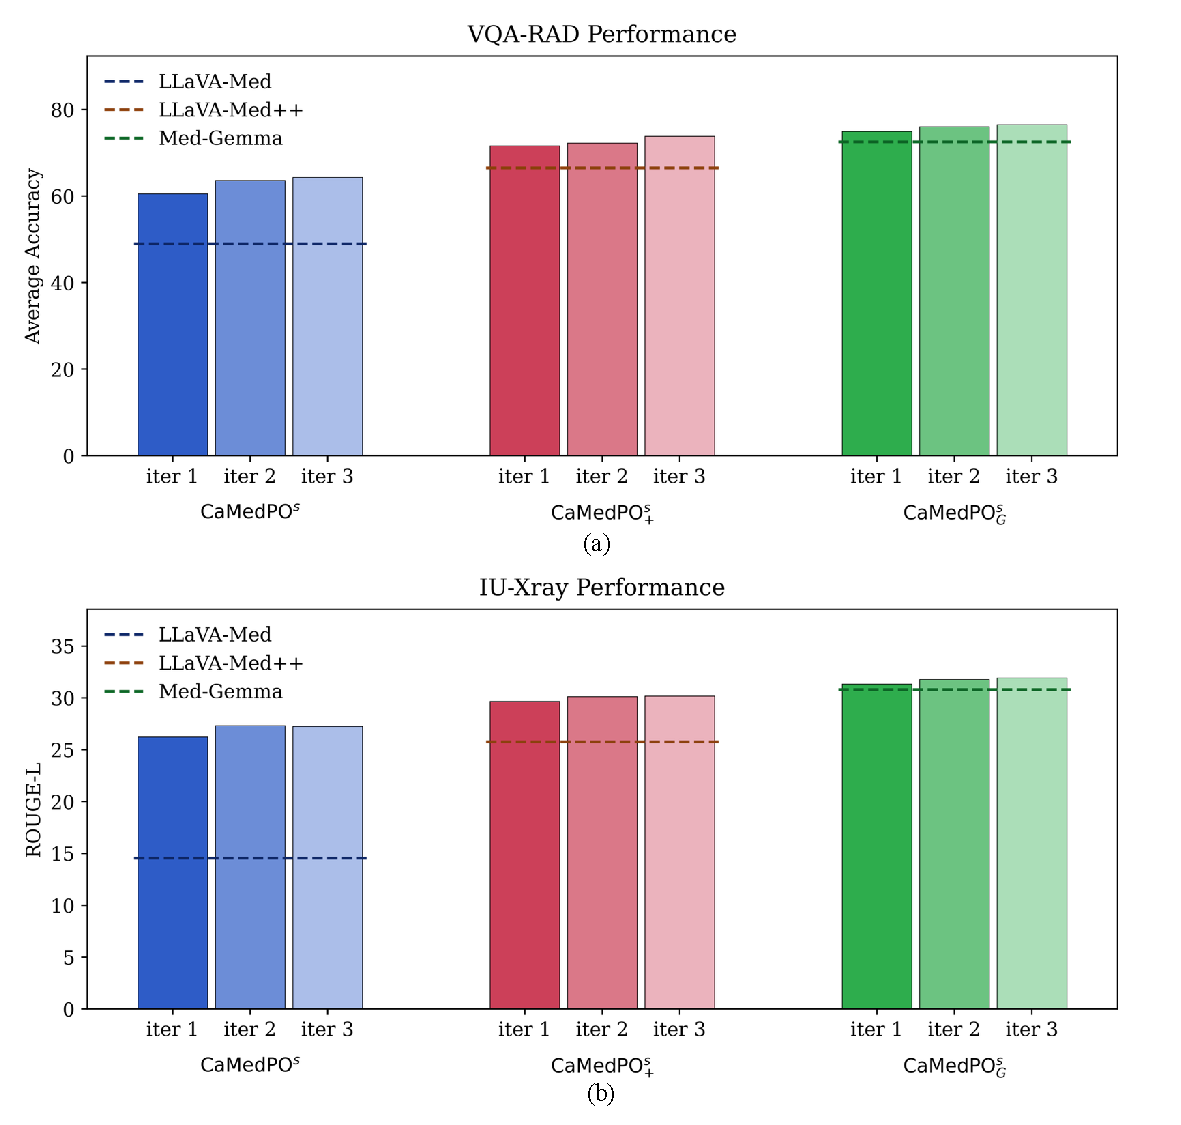
\includegraphics[width=1.0\linewidth]{figs/supp_ablation.pdf}
    \caption{Additional ablation study results on VQA-RAD and IU-XRay. $^\text{s}$ denotes the model enhanced with SFT. $_\text{+}$ denotes the baseline model is LLaVa-Med++, while $_\text{G}$ denotes the baseline model is Med-Gemma.}
    \label{fig:supp_ablation}
\end{figure}



\noindent\textbf{Multi-round Training.} In the multi-round training setup, each round initializes from the model obtained in the previous round and further refines its reasoning ability. On VQA-RAD, CaMedPO$^{s}$ improves over its baseline LLaVA-Med in every round, increasing from 60.53\% to 63.63\% and 64.30\%, while the baseline remains at 49.00\%. This demonstrates that our method can continuously correct the undesired biases inherited from the initial model. For better baseline models, such as LLaVA-Med++ and Med-Gemma, a single round of training already brings substantial gains, while the subsequent training can not benefit much. Overall, the multi-round pattern shows that our approach is particularly effective at correcting models with more severe biases.


\noindent\textbf{Compatibility Analysis on Other LVLMs.}
We further extend our preference optimization framework to two stronger medical LVLMs, LLaVA-Med++ and Med-Gemma, and use them as baselines for evaluating the general applicability of our method. On VQA-RAD, CaMedPO$^{s}_{+}$ improves over LLaVA-Med++ from 66.52\% to 71.62\% after the first optimization round. Similarly, CaMedPO$^{s}_{G}$ enhances Med-Gemma from $72.54$ to $74.94$ in the first round. These results demonstrate that our approach is not limited to a specific LVLM architecture and can reliably boost performance across different baselines. Although the improvements on Med-Gemma are relatively smaller compared to LLaVA-Med, this trend is expected. Med-Gemma has undergone large-scale pretraining on diversified medical and general-domain datasets, which reduces part of the shortcut bias and leaves less room for preference-based correction. This observation suggests that as LVLMs grow in scale and diversity, further progress may require deeper incorporation of disease mechanisms and medically grounded causal structures to guide both reasoning and training. Overall, the results confirm the broad compatibility of our method and highlight its effectiveness across LVLMs with varying bias levels and training regimes.

\begin{table}[t]
\centering
\caption{Performance analysis of sample ratio of causal pairs on VQA-RAD and IU-Xray.}
\label{tab:ratio_ablation}

\resizebox{\linewidth}{!}{
\setlength{\tabcolsep}{8pt}
\begin{tabular}{c cc ccc}
\toprule
\multirow{2}{*}{Ratio} &
\multicolumn{2}{c}{VQA-RAD} &
\multicolumn{3}{c}{IU-Xray} \\
\cmidrule(lr){2-3} \cmidrule(lr){4-6}
& Open & Closed & BLEU & ROUGE-L & METEOR \\
\midrule
0    & 37.00 & 67.73 & 24.00 & 30.13 & 35.17 \\
0.5  & 41.00 & 69.72 & 25.56 & 32.81 & 37.32 \\
0.75 & 44.00 & 72.11 & 26.43 & 33.76 & 38.05 \\
1.0  & 42.50 & 74.90 & 26.23 & 34.13 & 38.25 \\
1.25 & 39.00 & 73.70 & 25.12 & 30.83 & 36.07 \\
\bottomrule
\end{tabular}
}
\end{table}



\noindent\textbf{Sample Ratio of Causal Pairs.} In this section, we explore the how the ratio of the integrated causal preference loss affects the performance. In table \ref{tab:ratio_ablation}, a ratio of zero corresponds to the unweighted MMedPO objective, which yields the lowest performance across both VQA-RAD and IU-Xray. Introducing moderate causal weighting leads to consistent improvements. In particular, the ratio of one achieves the best overall performance, reaching 42.50\% and 74.90\% on VQA-RAD open and closed questions. When the ratio becomes larger, performance begins to drop. This decline indicates that overly amplifying the causal preference term may distort the balance between the original input semantics and the causal correction, ultimately limiting the model's reasoning capability. Overall, the results demonstrate that incorporating causal preference signals is beneficial, but the weighting must be properly calibrated to maintain stable and effective optimization.


\subsection{VQA Case Studies}

\subsubsection{Open-ended VQA Examples}

Figure~\ref{fig:open_vqa_cases} presents qualitative comparisons on open-ended medical VQA tasks. We observe that our causality-aware approach produces more clinically accurate responses by correctly identifying anatomical structures while baseline methods generate incorrect explanations based on spurious correlations.

\begin{figure}[ht]
\centering

\includegraphics[width=0.4\textwidth]{figs/case/3.pdf}
\caption{\textbf{Open-ended VQA case studies.} Comparison of responses from baseline methods and our causality-aware approach on challenging open-ended medical questions. Green checkmarks indicate clinically accurate anatomical identifications, while red thumb down icons denote factual errors or hallucinations.}
\label{fig:open_vqa_cases}
\end{figure}

In the presented case study, when asked ``What are the white spots in the black part of the lower part of body?" in a chest X-ray image, the baseline methods incorrectly attribute the visual features to ``the presence of air" with lengthy, confidence-based explanations. In contrast, our causality-aware approach correctly identifies the anatomical structures as ``Lung" and ``Pulmonary Bronchus" with concise, medically accurate responses. This demonstrates how our method focuses on medically relevant visual evidence while avoiding the spurious correlations that lead baseline methods to generate clinically inaccurate explanations about air presence when the actual question pertains to identifiable anatomical structures in the thoracic cavity.

\subsubsection{Close-ended VQA Examples}

Figure~\ref{fig:close_vqa_cases} illustrates performance on close-ended medical VQA tasks, where our causality-aware approach demonstrates superior accuracy in medical abnormality detection compared to baseline methods.

\begin{figure}[ht]
\centering

\includegraphics[width=0.4\textwidth]{figs/case/6.pdf}
\caption{\textbf{Close-ended VQA case studies.} Binary medical questions where our causality-aware approach correctly identifies normal anatomical structures while baseline methods incorrectly detect non-existent abnormalities. Green checkmarks indicate clinically accurate anatomical identifications, while red thumb down icons denote factual errors or hallucinations.}
\label{fig:close_vqa_cases}
\end{figure}

In the presented case study, when asked ``Is there any abnormality in the spleen?" regarding an MRI image showing an axial abdominal slice, our causality-aware approach correctly answers ``No" (indicating no splenic abnormality) with concise, confident responses. In contrast, baseline methods incorrectly respond ``Yes" and proceed to hallucinate detailed descriptions of non-existent ``splenic masses" and ``abnormal growths." This demonstrates how our causal reasoning framework prevents false positive detections that commonly plague traditional medical VQA systems, ensuring clinical decisions are based on accurate visual evidence rather than spurious pattern correlations.

\subsection{Report Generation Case Studies}

Figure~\ref{fig:report_generation} demonstrates qualitative improvements in chest X-ray report generation, where our causality-aware approach shows superior performance in identifying complex pathological findings compared to baseline methods.

\begin{figure}[ht]
\centering

\includegraphics[width=0.4\textwidth]{figs/case/1.pdf}
\caption{\textbf{Medical report generation case studies.} Comparative analysis of chest X-ray report quality, highlighting our method's ability to accurately identify complex pathological findings while baseline methods either miss critical findings or provide incomplete assessments. Green checkmarks indicate accurate pathological identifications, while orange checkmarks denote partial accuracy, and thumb down icons represent missed diagnoses.}
\label{fig:report_generation}
\end{figure}

In the presented case study, when instructed to ``review the chest X-ray image and create a report that assesses any abnormalities, including potential signs of old empyema, fractures, or other abnormalities in the thoracic cavity," our causality-aware approach correctly identifies the complex pathology including ``Large right-sided pleural effusion with associated atelectasis. Cardiomegaly with pulmonary edema." In contrast, baseline methods demonstrate significant limitations: one method completely misses all pathological findings and incorrectly reports "Normal chest X-ray. Clear lungs. Heart size normal, ``while another provides only partial assessment by identifying ``Right pleural effusion" and ``some pulmonary vascular congestion" but fails to recognize the full extent of cardiomegaly and pulmonary edema. This case exemplifies how our causal reasoning framework enables comprehensive pathological assessment, ensuring that critical findings such as pleural effusions, cardiac enlargement, and pulmonary vascular changes are accurately identified and properly described in the generated medical reports.



\section{Related Works}
\label{supp:related}
\textbf{Preference Optimization for LMs/LVLMs.}
Preference optimization is widely used to align large vision–language models (LVLMs) with human or model preferences~\cite{ouyang2022training, liu2025survey}. 
Early work on reinforcement learning from human feedback (RLHF) \cite{Christiano2017RLHF} trains a reward model from human comparisons and optimizes a policy via proximal policy optimization (PPO) \cite{Schulman2017PPO}, whereas Direct Preference Optimization (DPO) \cite{rafailov2023direct} replaces the RL stage with a closed-form Bradley–Terry model \cite{Bradley1952BT} which improves efficiency and stability. 
Subsequent variants refine the DPO objective through margin-based, utility-based, or sampling-based strategies (KTO \cite{Ethayarajh2024KTO}, RSO \cite{liustatistical}, ORPO \cite{hong2024reference}), while methods such as SimPO \cite{meng2024simpo} and SPPO \cite{wu2025selfplay} further simplify alignment by removing explicit reward modeling or generating preferences via self-play. 
In multimodal setting, mDPO \cite{wang2024mdpo} extends DPO with conditional visual inputs (multi-view or multi-region), showing how pair construction and conditioning choices affect alignment. 
Our approach remains within the direct optimization family but introduces causal-aware sample weighting to better exploit clinically relevant visual evidence.